\documentclass{article}
%\usepackage[a4paper, total={6in, 8in}]{geometry}
\usepackage{geometry}
 \geometry{
 a4paper,
 total={210mm,297mm},
 left=20mm,
 right=20mm,
 top=-2mm,
 bottom=2mm,
 }
%\usepackage[margin=0.5in]{geometry}
\usepackage{float}
\usepackage{subfig}
\usepackage{amsmath,amssymb}
\usepackage{ifpdf}
%\usepackage{cite}
\usepackage{algorithmic}
\usepackage{array}
\usepackage{mdwmath}
\usepackage{pdfpages}
\usepackage{mdwtab}
\usepackage{eqparbox}
\usepackage{cite}
%\onecolumn
%\input{psfig}
\usepackage{color}
\usepackage{graphicx}
\setlength{\textheight}{23.5cm} \setlength{\topmargin}{-1.05cm}
\setlength{\textwidth}{6.5in} \setlength{\oddsidemargin}{-0.5cm}
\renewcommand{\baselinestretch}{1}
\pagenumbering{arabic}
\usepackage{ragged2e}
\renewcommand{\baselinestretch}{1.358}
\graphicspath{ {./images/}}


\begin{document}

\textbf{
\begin{center}
{
\large{School of Engineering and Applied Science (SEAS), Ahmedabad University}\vspace{3mm}
}
\end{center}
%
\begin{center}
\large{B.Tech(CSE) Semester IV: Probability and Stochastic Processes (MAT 277) }\\ \vspace{2mm}
\end{center}
}
\begin{itemize}
\item Group No : BB14
\item Group Members : \\ Jinesh Salot (AU1940178), Kathan Shah (AU1940152), Nipun Patel (AU1940033), Poojan Gandhi (AU1940125), Rohan Parikh (AU1940157), Samkit Kundalia (AU1940021), Tirth Patel (AU1940137)
 %\item Roll no: s1749002 (Ph.d)
%\item Associated with Project: DST-UKIERI
\item Project Title: Probabilistic distribution of births over a certain period of time 
\end{itemize} 

\section {Justify how Probabilistic Models are used in your project. How is uncertainty modeled?}
{The aim of our project was to estimate the probability of at-least {\slshape r} live births in given span of time and the mean difference between two live births. Probability concepts used for our modelling are {\slshape Binomial Distribution, Geometric Distribution, Poisson Distribution, Probability Mass Function (PMF) and Cumulative Mass Function (CMF).}\\

The Coital Frequency is modelled using {\slshape Poisson Random Variable}. Its {\slshape lambda} will be the mean daily probability of intercourse in a month of 30 days. The fertile period is considered to be 4-5 days. The probability of fetal loss is considered to be fixed in order to find the pregnancy leading to live birth for different intervals of time (in years). \\

Probability of conception is assumed to be fixed in the base article but we have modelled it using {\slshape Geometric Distribution, PMF and CMF} as part of our innovation work. Using {\slshape Binomial Distribution} where probability of success is the probability of conception and using {\slshape Cumulative Distribution Function} over all ranges of {\slshape X} and {\slshape v} where is {\slshape X} describes the event of a live birth and {\slshape v} describes the event of a fetal loss.}\\
\begin{center}
	{\large {\bfseries Modelling of Uncertainties}}
\end{center}
Many uncertain events occur before, during and after pregnancy like the {\slshape Coital Frequency}, {\slshape Fertile Period during Menstrual Cycle} , {\slshape Conception}, {\slshape Fetal Losses}, {\slshape Number of births over a certain period of time.}\\

The Coital Frequency is modelled using {\slshape Poisson Random Variable} and {\slshape $\lambda$} will be the mean daily probability of intercourse in a month of 30 days. The fertile period is considered to be 4-5 days. The probability of fetal loss is considered to be fixed in order to find the pregnancy leading to live birth for different intervals of time (in years).\\

Probability of conception is assumed to be fixed in the base article but we have modelled it using {\slshape Geometric Distribution, PMF} and {\slshape CMF} as part of our innovation work. Using {\slshape Binomial Distribution} where probability of success is the probability of conception and using {\slshape Cumulative Distribution Function} over all ranges of {\slshape X} and {\slshape v} where as {\slshape X} describes the event of a live birth and {\slshape v} describes the event of a fetal loss, we modelled the probability of at-least {\slshape r} live birth in a {\slshape t} given years over various mortality rates. Also our model estimates the mean difference between two live births in a span of different {\slshape t} years.\\

%Pregnancy outcomes are uncertain in nature, that depend on a lot of factors like: coital frequency,
%susceptibilty,
%probability of conception,
%use of contraceptives,
%probability of fetal loss,
%number of births over a period of time,
%fecundability and
%fertility period and length of menstrual cycle etc. \\
%To ascertain the Conception Probability - we modelled it as a {\slshape Binomial Random Variable}.
%We considered the probability of fetal losses to be fixed by deciding the mortality rate for the fetuses in order to find the pregnancy leading to Live Birth for different intervals of time. We also found the mean interval of months, that is the difference between two live births for the total period of 10,15 years etc.\\
%We were able to model the probability of {\itshape r} numbers of live births given the probability of fetal mortality over the span of {\itshape t} years. Our model also estimates the mean difference between two live births in a span of different {\slshape t} years.

\section{Clearly enlist the new things done in the coding part, excluding the shared code.}

%\begin{enumerate}
%    %\item Mention code change-1
%    \item Modelled probability of conception which previously the author had taken constant. We did it using concepts of conditional probability and binomial random variables.
%    \item Used coital frequency, number of fertile days, coital frequency between fertile days and days of intercourse occurred in fertile period as parameter to find probability of conception which was taken constant by author previously.
%    \item Tuned the authors model to find the probability of exactly r fetal loss in a period of y years.
    %\item {\large TOBEDONE} %TO BE DONE AEZ 4th Point
    {\large Code Changes -1}
\begin{itemize} 
	\item Probability of conception is taken constant in the base paper assuming they have used contraceptives. So we have modelled the probability of conception as our innovation part. 
	\item We have taken certain new parameters like coital frequency, fertile period, menstrual cycle length, no. of coital acts during fertile period, no. of days when at least one coital act happened in the fertile period, Prob. of fetal loss.
	\item Based on those parameters we modelled the probability conception for low, intermediate and high cycle based on the cycle length and from that we have estimated the effective probability of conception (fecundability). 
	\item That probability we have used in our main model and find the probability of at-least r live birth in t years of time and plotted the graph for the same.	
\end{itemize}
{\large Code Changes -2}
\begin{itemize}
	\item In the base paper the author varies the number of fetal loss over a period of time and derives the probability of r births in y years. By taking the similar approach as the author we varied the number of births over the period of time to get the probability mass function of fetal loss.
\end{itemize}
{\large Code Changes -3}
\begin{itemize}
	\item We have estimated the mean month for the occurrence of r-live birth. For that we have taken into account the gestation period and   postpartum in-fecundability period to be constant.
	\item From that we have estimated the mean difference between two live births in terms of months. 
\end{itemize}

%\end{enumerate}
\section{Contribution of team members}	
\subsection{Technical contribution of all team members }
\begin{table}[H]
\centering
\begin{tabular}{|m{3.8154cm}|m{1.4154cm}|m{1.4154cm}|m{1.4154cm}|m{1.4154cm}|m{1.4154cm}|m{1.4154cm}|m{1.4154cm}|}
\hline
Tasks  & Jinesh Salot & Kathan Shah & Nipun Patel & Poojan Gandhi & Rohan Parikh & Samkit Kundalia & Tirth Patel \\ \hline
Recreating Results of Base Paper &  {\Large \checkmark}    & {\Large \checkmark}      & {\Large \checkmark}       & {\Large \checkmark}         & {\Large \checkmark}    &  {\Large \checkmark}     &  {\Large \checkmark}       \\ \hline
Coding for Innovation Part &    {\Large \checkmark}  &       &  {\Large \checkmark}      &   {\Large \checkmark}       &     &    & {\Large \checkmark}        \\ \hline
Integrating Innovation into the existing model &      &  {\Large \checkmark}     &        &   {\Large \checkmark}       & {\Large \checkmark}    &  {\Large \checkmark}     &  {\Large \checkmark}     \\ \hline
\end{tabular}
\end{table}
\subsection{Non-Technical contribution of all team members }
\begin{table}[H]
		\begin{tabular}{|p{3.8154cm}|p{1.4154cm}|p{1.4154cm}|p{1.4154cm}|p{1.4154cm}|p{1.4154cm}|p{1.4154cm}|p{1.4154cm}|}
		%\begin{tabular}{|l|l|l|l|l|l|l|l|}
			\hline
			Tasks  & Jinesh Salot & Kathan Shah & Nipun Patel & Poojan Gandhi & Rohan Parikh & Samkit Kundalia & Tirth Patel \\ \hline
			Research for Innovation &  {\Large \checkmark}    & {\Large \checkmark}      &{\Large \checkmark}        &  {\Large \checkmark}        & {\Large \checkmark}    &   {\Large \checkmark}    &  {\Large \checkmark}       \\ \hline
			Concept Map -1 &   {\Large \checkmark}   &  {\Large \checkmark}     &        &   {\Large \checkmark}       &     &      &  {\Large \checkmark}       \\ \hline
			Meeting with Medical Experts &      &  {\Large \checkmark}     &    {\Large \checkmark}    &          &   {\Large \checkmark}  &   {\Large \checkmark}    &       \\ \hline
			Report & {\Large \checkmark}     &       &   {\Large \checkmark}     &          & {\Large \checkmark}    &  {\Large \checkmark}     & {\Large \checkmark}      \\ \hline
		\end{tabular}
\end{table}


\section{Any innovation done considering the society/neighborhood problem?}
After consulting medical professionals for the project, we got to know their perspective and how serious the issue is. We also interacted with a couple who faced an undesirable pregnancy outcome. This is a very serious yet less talked about problem because of the sensitivity involved. \\

We realised that in our case study, between the theoretical models and practical results - there were vast differences. Due to the complexity of many factors involved - the base paper assumed many of them to be constant. However, we wanted to try to minimize the gap between reality and theory as much as possible.\\

Family planning is always something that is of vital importance to any couple. A part of our model also focuses on the effect of using contraceptives for couples. The following are the quantified results of our learnings: \\ 

\begin{figure}[H]%
	\centering
	\subfloat[\centering Probability of Conception=0.01 (Using Contraceptive)(From Base Article)]{{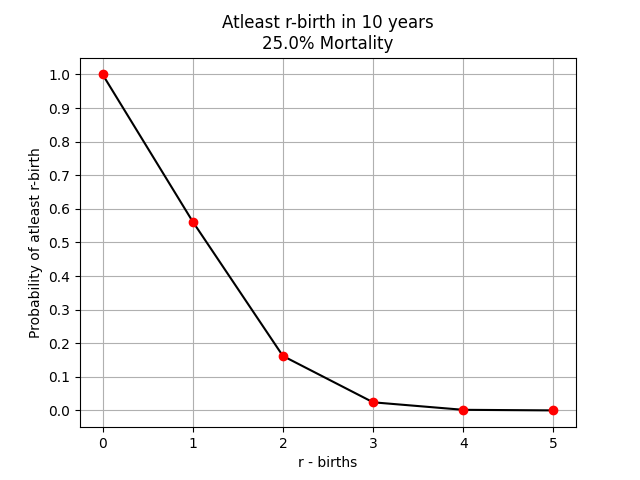
\includegraphics[width=7cm]{atleast_10years_25_alpha.png} }}%
	\qquad
	\subfloat[\centering Probability Of Conception = 0.27 (Derived from Model)(Innovation work)]{{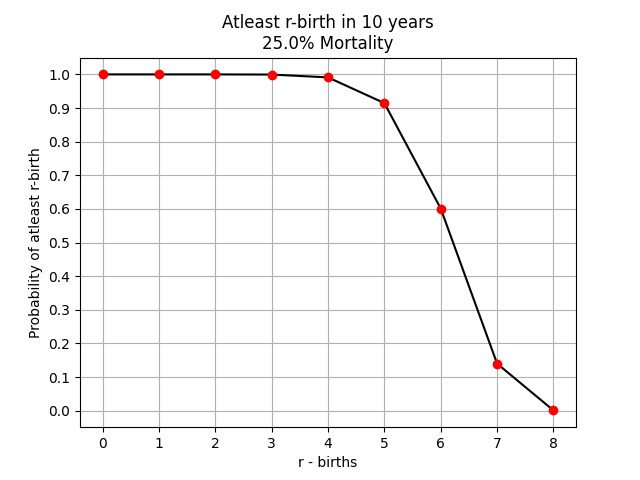
\includegraphics[width=7cm]{innovation_atleast_10years_25_alpha.png} }}%
	\caption{Side-by-side comparison of effect on Pregnancy upon using Contraceptions}%
	\label{fig:example}%
\end{figure}

We hope our effort to solve this problem serves as a pillar to future studies and groups in understanding it. With further research and understanding of interdisciplinary domains surrounding it - we believe that, our model can be of vital importance to the society. The immediate benefit of our work can be taken advantage of by stakeholders like patients, doctors, gynaecologists, obstetricians and medical societies and institutions.\\

\section{Enumerate the inferences derived from user-centric perspective.}
We find the probability of conception using the length of the cycle, number of fertile days in that cycle and number of coital acts in that cycle as a factor. This will be useful to couples for family planning by calculating the probability of conception when they use contraceptives.\\

We have calculated the mean number of months between two live births given the probability of conception (considering that the couple is using contraceptives) taking the mortality rate of fetuses as a factor. This would be useful to couples who use contraceptives and want to know the chances of the number of births of the child and also the time interval of birth between them even after using contraceptives.\\
	\begin{table}[H]
		\begin{center}
			\begin{tabular}{|m{2.4154cm}|m{6.4154cm}|m{6.4154cm}|}
				\hline
				Fetal Mortality Rate  & Mean number of months between two livebirths(Base Paper) & Mean number of months between two livebirths (New Model)\\ \hline
				0\% & 114    &17.701 \\ \hline
				10\% & 125.6 &18.6681 \\ \hline
				25\% & 148.7 &20.6018 \\ \hline
			\end{tabular}
		\end{center}
	\end{table}


\begin{enumerate}
\item Even after using the contraceptive, couples should at least expect 1 child as the expected values of births are 1.5, 1.4 and 1.2 for probability of fetal mortality=0,0.1,0.25.
\item For couples who want to have a child there is a 20\% chance that over a 15 year period they will have 2 or 3 Stillbirths/Miscarriages.
\item By modelling the probabilities of r births in y years we can see that even using contraceptives (thus reducing the probability of conception to 0.01) for a period of 10 years there is 0.6273 probability that at least 1 child is born.
\end{enumerate} 

\section{References}


\bibliographystyle{IEEEtran}
\bibliography{ref.bib}

\end{document} 